\documentclass[a4paper,12pt]{article}
\usepackage[a4paper,top=1.3cm,bottom=2cm,left=1.5cm,right=1.5cm,marginparwidth=0.75cm]{geometry}
\usepackage{setspace}
\usepackage{cmap}
\usepackage{mathtext}
\usepackage[T2A]{fontenc}
\usepackage[utf8]{inputenc}
\usepackage[english,russian]{babel}
\usepackage{multirow}
\usepackage{graphicx}
\usepackage{wrapfig}
\usepackage{tabularx}
\usepackage{float}
\usepackage{longtable}
\usepackage{hyperref}
\hypersetup{colorlinks=true,urlcolor=blue}
\usepackage[rgb]{xcolor}
\usepackage{amsmath,amsfonts,amssymb,amsthm,mathtools}
\usepackage{icomma}
\mathtoolsset{showonlyrefs=true}
\usepackage{euscript}
\usepackage{mathrsfs}
\usepackage{float}
\setlength{\parindent}{1.5cm} % Устанавливает отступ в 1.5 см для всех абзацев


\DeclareMathOperator{\sgn}{\mathop{sgn}}
\newcommand*{\hm}[1]{#1\nobreak\discretionary{}
	{\hbox{$\mathsurround=0pt #1$}}{}}

\title{\textbf{Отчёт о выполненой лабораторной работе \\ \textit{Измерение коэффициента поверхностного натяжения жидкости (2.5.1)}}}
%\title{\textit{}{Измерение удельной теплоёмкости воздуха при постоянном давлении (2.1.1)}}
\author{Каплин Артём Б01-402}
\date{16 февраля 2025}

\begin{document}

\maketitle

	\section{Аннотация}

	\textbf{Цель работы:} 1) измерение температурной зависимости  коэффициента поверхностного натяжения дистиллированной воды с использованием известного коэффициента поверхностного натяжения спирта;  2) определение полной поверхностной энергии  и теплоты, необходимой для изотермического образования единицы  поверхности жидкости  при различной температуре. \\
\newline
	\textbf{Оборудование:} прибор Ребиндера с термостатом и микроманометром;
исследуемые жидкости; стаканы.

	\section{Теоретические сведения}
    \subsection{Термодинамика поверхностного натяжения}
    \textit{Поверхностным натяжением} называется изотермическая работа, которую надо затратить, не меняя объёма жидкости, чтобы увеличить поверхность на единицу. Коэффициент поверхностного натяжения как обозначается $\sigma$.
Коэффициент поверхностного натяжения равен силе, действующей на единицу длины контура поверхности жидкости. Эта сила направлена вдоль поверхности перпендикулярно линии контура.
\begin{equation*}
	\sigma = \frac{f}{L}
	\eqno(1)
\end{equation*}
\begin{equation*}
	\delta A_{T} = -\sigma d\Pi
\end{equation*}

\[
\Psi = U_{\text{п}} - TS - \text{свободная энергия}
\label{key}
\]
Использую первое и второе начало термодинамики, получим:
\begin{equation*}
	\delta Q = dU_{\text{п}}-\sigma d\Pi,
        \eqno(2)
\end{equation*}
\begin{equation*}
	dU_{\text{п}} = TdS + \sigma d\Pi,
	\eqno(3)
\end{equation*}
Теперь продифференцируем выражение с свободной энергией и подставим туда выражение (3):

\[
    d\Psi_{\text{п}} = dU_{\text{п}} - SdT - TdS = TdS + \sigma d\Pi - SdT - TdS = -SdT + \sigma d\Pi
\]
Из предыдущего выражения получем:
\begin{equation*}
	S = - (\frac{\partial \Psi_{\text{п}}}{\partial T})_{\Pi},
	\eqno(4)
\end{equation*}
\begin{equation*}
	\sigma = (\frac{\partial \Psi_{\text{п}}}{\partial \Pi})_{T}.
	\eqno(5)
\end{equation*}
Интегрируя последнюю формулу, полагая, что при $\Psi_{\text{п}} = 0$, $\Pi = 0$, получаем
\begin{equation*}
	\Psi_{\text{п}} = \sigma \Pi.
	\eqno(6)
\end{equation*}

Теперь мы можем получить соотношение для внутрненней поверхности слоя жидкости:
\[
    U_{\text{п}} = \Psi_{\text{п}} + TS = \sigma \Pi + T(-\frac{d \sigma}{dT}\Pi) = (\sigma - T\frac{d \sigma}{dT})\Pi
\]
Поскольку процесс расширения плёнки изотермический, то теплота, сообщаемая пленке при её расширении от площади $\Pi_1$ до $\Pi_2$ равна:
\[
    Q_T = T\left[ S(T, \Pi_2) - S(T,\Pi_1)\right] = -T\frac{d \sigma}{dT}(\Pi_2 - \Pi_1)
\]
где теплотой образования единицы поверхности назыввется:
\[
    q = -T\frac{d \sigma}{dT}
\]
    Наличие поверхностного слоя приводит к различию давлений по разные стороны от искривленной границы раздела двух сред.  Для сферического пузырька с воздухом  внутри жидкости избыточное давление дается формулой Лапласа:

	\begin{equation}
		\Delta P = P_{\text{внутри}} - P_{\text{снаружи}} = \frac{2\sigma}{r},
		
	\end{equation}
	где $ \sigma $ -- коэффициент поверхностного натяжения, $ P_{\text{внутри}} $ и $ P_{\text{снаружи}} $ -- давление внутри пузырька и снаружи, $ r $ -- радиус кривизны поверхности раздела двух фаз. Эта формула лежит в основе предлагаемого метода определения коэффициента поверхностного натяжения жидкости. Измеряется давление $ \Delta P $, необходимое для выталкивания в жидкость пузырька воздуха.

    \section{Экспериментальная установка}

    \begin{figure}[!ht]
        \begin{center}
            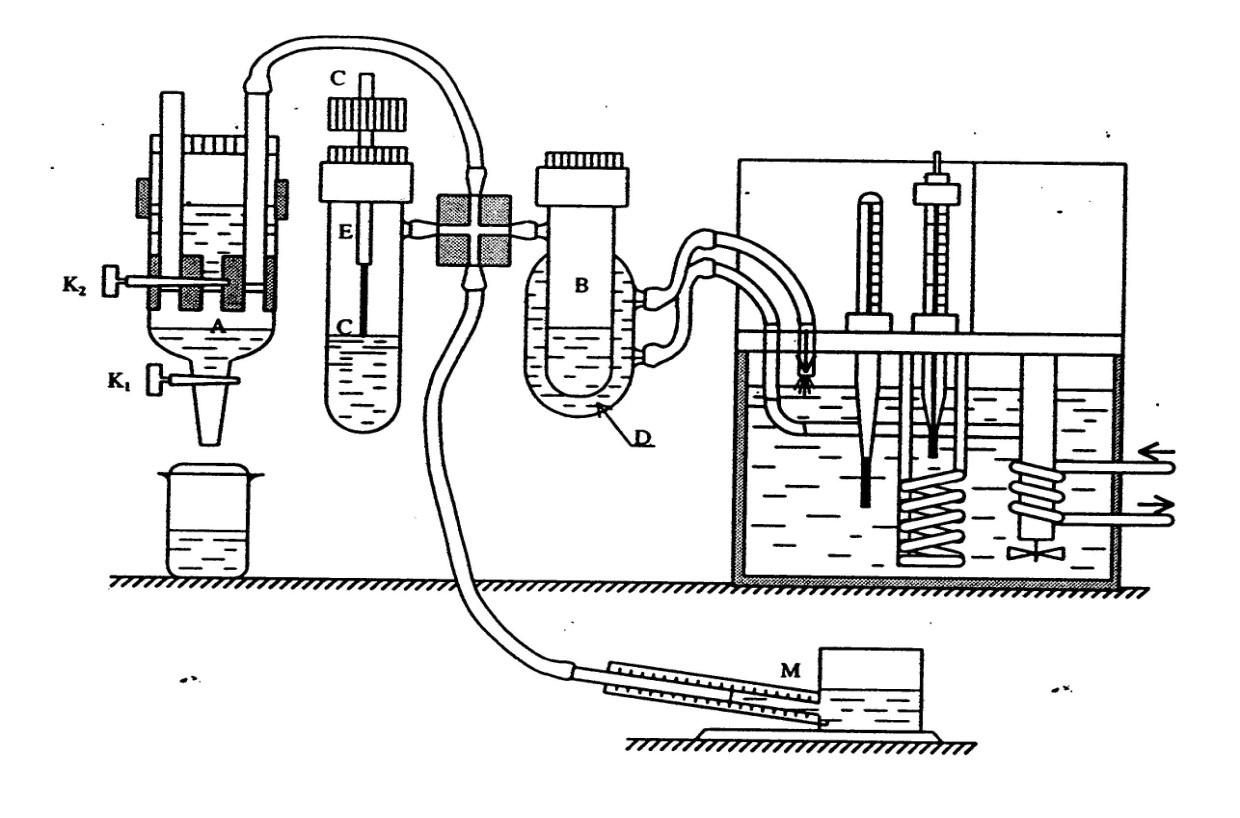
\includegraphics[width=0.6 \textwidth]{ust.jpg}
        \end{center}
        \caption{Экспериментальная установка}
                \label{img:ust}
    \end{figure}

    Исследуемая жидкость (дистиллированная вода) наливается в сосуд (колбу) $ B $ (рис. \eqref{img:ust}). Тестовая жидкость  (этиловый спирт) наливается  в сосуд $ E $.  При измерениях  колбы герметично закрываются  пробками. Через одну из двух пробок  проходит полая металлическая игла $ С $. Этой пробкой закрывается сосуд, в котором  проводятся измерения. Верхний конец иглы открыт в атмосферу, а нижний погружен в жидкость. Другой сосуд герметично закрывается второй пробкой. При создании достаточного  разряжения воздуха в колбе с иглой пузырьки воздуха начинают пробулькивать через жидкость. Поверхностное натяжение можно определить по величине разряжения $ \Delta P $ \eqref{key}, необходимого для прохождения пузырьков (при известном радиусе иглы).

	Разряжение в системе создается с помощью аспиратора $ A $. Кран $ K_2 $ разделяет две полости аспиратора. Верхняя полость при закрытом кране $ K_2 $ заполняется водой. Затем кран $ K_2 $ открывают и заполняют водой  нижнюю полость  аспиратора.  Разряжение воздуха создается в нижней полости  при открывании крана $ K_1 $, когда  вода вытекает из неё по каплям. В колбах $ В $ и $ С $, соединённых трубками с нижней полостью аспиратора, создается такое же пониженное давление. Разность давлений в полостях с разряженным воздухом и атмосферой измеряется спиртовым микроманометром.

	Для стабилизации температуры исследуемой жидкости через рубашку $ D $ колбы $ В $ непрерывно прогоняется вода из термостата.

	Обычно кончик иглы лишь касается поверхности жидкости, чтобы исключить влияние гидростатического давления столба жидкости. Однако при измерении температурной зависимости коэффициента поверхностного натяжения возникает ряд сложностей. Во-первых, большая теплопроводность металлической трубки приводит к тому, что температура на конце трубки заметно ниже, чем в глубине жидкости. Во-вторых, тепловое расширение поднимает уровень жидкости при увеличении температуры.

	Обе погрешности можно устранить, погрузив кончик трубки до самого дна. Полное давление, измеренное при этом микроманометром, равно \[ P = \Delta P + \rho g h.\] Заметим, что $ \rho gh $ от температуры практически не зависит, так как подъём уровня жидкости компенсируется уменьшением её плотности (произведение $ \rho g $ определяется массой всей жидкости и поэтому постоянно). Величину  $ \rho g h $ следует измерить двумя способами.

	Во-первых, замерить величину $ P_1= \Delta P' $, когда кончик трубки только касается поверхности жидкости. Затем при этой же температуре опустить иглу до дна и замерить $ P_2= \rho gh + \Delta P'' $ ($ \Delta P' $, $ \Delta P'' $ -- давление Лапласа). Из-за  несжимаемости  жидкости можно положить $ \Delta P' = \Delta P'' $ и тогда \[ \rho gh= P_2 - P_1. \]

	Во-вторых, при измерениях $ P_1 $ и $ P_2 $ замерить линейкой  глубину погружения иглы $ h $. Это можно сделать, замеряя расстояние между верхним концом иглы и любой неподвижной частью прибора при положении иглы на поверхности и в глубине колбы.


    \section{Ход работы}

    \subsection{Проверка герметичности установки}
    Для проверки опускаем чистую сухую иглу в сосуд со спиртом так, чтобы кончик иглы лишь касался поверхности спирта. Плотно закрываем обе колбы и открываем кран аспиратора для пробулькивания пузырьков воздуха в колбе. Замеряем показания микроманометра, они не должны меняться.

		\subsection{Начало измерений}

			Положением крана аспиратора подбираем частоту падения капель так, чтобы максимальное давление манометра не зависело от этой частоты (не чаще чем 1 капля в 5 секунд).

		\subsection{Определение диаметра иглы}
			\label{needle_diam}

			Параметры при измерениях:

			\begin{align*}
				t_{комн} &= 22,3~^oC & \sigma_{спирт} &= 22.78~\frac{\text{мН}}{\text{м}}
			\end{align*}

			Измеряем максимальное давление $\Delta P_{спирт}$ при пробулькивании пузырьков воздуха через спирт.
                Провели 5 измерений. Показания манометра для всех $h_{ман} = 49,5 \text{мм}$. Значит случайная погрешность измерений равна 0. То есть погрешнсть измерений будет определятся погрешностью микроманометра (класс точности --- 1,0):

                \[
                \Delta P = C \cdot h \cdot \frac{\gamma_{\text{сп. залит.}}}{\gamma_{\text{сп.пр.}}} \cdot K \cdot 9,81 = (97,119 \pm 1,94) \  \text{Па} 
                \]
                где C = 1,00 --- поправочный множитель; K = 0,2 --- постоянная угла наклона; $\gamma_{\text{сп. залит.}} = 0,8095$ --- плотность прибора, залитого в прибор; $\gamma_{\text{сп.пр.}} = 0,8095$ --- плотность спирта, указанная на прибора
                \[
                d = \frac{4 \sigma_{\text{спирт}}}{\Delta P} = (0,938 \pm 0,0187) \ \text{мм}
                \]


			Измеряем диаметр внутреннего отверстия иглы при помощи микроскопа: \\ $d_{\text{микроскоп}} = (1,05 \pm 0,05) \text{мм}$ \\

            Результат, измеренный микроскопом больше экспериментального значения на $0,122 \ \text{мм}$. Такое расхождение можно объяснить несколькими причинами:
			\begin{itemize}
				\item во время эксперимента за короткий промежуток времени из иглы пробулькивало сразу по 2 пузырька воздуха;
				\item игла может быть загрязнена жиром (или чем то другими).
			\end{itemize}
            Далее будем использовать диаметр иглы, измеренный микроскопом, как более точный.

            \subsection{Измерения для дистиллированной воды с иглой на поверхности}

			Промываем и просушиваем иглу. Далее приводим её в соприкосновение с поверхностью дистиллированной воды. Регулируем скорость поднятия уровня спирта в манометре и измеряем максимальное давление пробулькивания пузырьков $P_1$. Также измеряем расстояние между верхним концом иглы и неподвижным торцом сосуда $h_2$.

			\begin{align*}
				P_1 &= (229,5 \pm 4,6) \ \text{Па}\\
				h_1 &= (21,0 \pm 0.5) \ \text{мм}
			\end{align*}

                \subsubsection{Измерения для дистиллированной воды с погружённой иглой}

			Иглу опускаем максимально вниз. Измеряем расстояние $h_2$ как в предыдущем пункте. Посчитаем максимальное давление $P_2$.

			\begin{align*}
				P_2 &= (361,99 \pm 7,24)\ \text{Па}\\
				h_2 &= (7,5 \pm 0,5)\ \text{мм}
			\end{align*}

			По разности давлений $\Delta P = P_2 - P_1 = (132,49 \pm 2,65)\ \text{Па}$ определим глубину погружения $\Delta h$ иглы и сравним с $\Delta h = h_1 - h_2$. Плотность воды при комнатной температуре ($25^oC$) $\rho_{\text{вода}} = 997.0\ \frac{\text{кг}}{\text{м}^3}$


			\begin{align*}
				\Delta h &= \frac{\Delta P}{\rho_{вода} g} = (13,5 \pm 0.4)~мм\\
				\Delta h &= h_1 - h_2 = (13,5 \pm 0.5)~мм
			\end{align*}

                Значения $\Delta h$ полностью совпали.

		\subsection{Температурная зависимость $\sigma(T)$}

			Включаем термостат, надеваем рубашку на колбу с водой, чтобы уменьшить теплопотери, уходящие в окружающую среду. Дожидаемся установления температуры около $25^oC$ в течение 5 минут. Проводим несколько измерений давления. Далее снимаем показатели давления с микроманометра через каждые $\Delta T = 5\ K$.
            \[
            \sigma_P = P \sqrt{\left( \frac{\sigma_h}{h} \right)^2} = 3,69 \ \text{Па}
            \]

			Посчитали погрешность учитывая случайную. Результаты измерений приведены в таблице.\ref{tab:sigma_T}.

		\subsection{Расчёт величины коэффициента поверхностного натяжения}

			Посчитаем коэфициент поверхностного натяжения для каждой из температур, из уравнения (\ref{key}):

            \[
            \sigma = \frac{d_{\text{игла}} \cdot P}{4}
            \]
            
            \[
            \sigma_{\sigma} = \sigma \sqrt{\left( \frac{\sigma_P}{P} \right)^2 + \left( \frac{\sigma_d}{d} \right)^2} = 4.82 \ \text{мН/м}
            \]

			Результаты в таблице \ref{tab:sigma_T}.

			\begin{table}[!ht]
				\centering
				\begin{tabular}{|c|c|c|c|}
					\hline

					$T, K$ & $h, \text{мм}$ & $P, \text{Па}$ & $\sigma, \text{мН/м}$\\ \hline
					$298 \pm 2$ & $183,75 \pm 1$ & $360,52$  & $94,64 $\\ \hline
					  $303 \pm 2$ & $183,50 \pm 1$ & $360,03$  & $94,50 $\\ \hline
					  $308 \pm 2$ & $185,00 \pm 1$ & $362,97$  & $95,28 $\\ \hline
					  $313 \pm 2$ & $186,33 \pm 1$ & $365,59$  & $95,97 $\\ \hline
					  $318 \pm 2$ & $181.83 \pm 1$ & $356,76$  & $93,65 $\\ \hline
					  $324 \pm 2$ & $181,00 \pm 1$ & $355,12$  & $93,22 $\\ \hline
					$329 \pm 2$ & $181,50 \pm 1$ & $356,10$  & $93,48 $\\ \hline
					  $333 \pm 2$ & $180,50 \pm 1$ & $354,14$  & $92,96 $\\ \hline			
				\end{tabular}
				\caption{Результаты измерений зависимости $\sigma(T)$}
				\label{tab:sigma_T}
			\end{table}
                Результаты измерений оказались весьма неточными, это мы можем увидеть в таблице.
                Давление не падало равномерно с повышением температуры, его значения прыгали на микроманометре то вверх, то вниз. Установка была полностью проверена на корректность работы, однако это не помогло стабилизировать давление. Могу предположить, что это может быть связано с условиями перечисленными в пункте 4.3.

                \section{Построим графики различных зависимостей от температуры}
                \subsubsection{График зависимости температуры от коэффициента поверхностного натяжения}

                 \begin{figure}[!ht]
                    \begin{center}
                        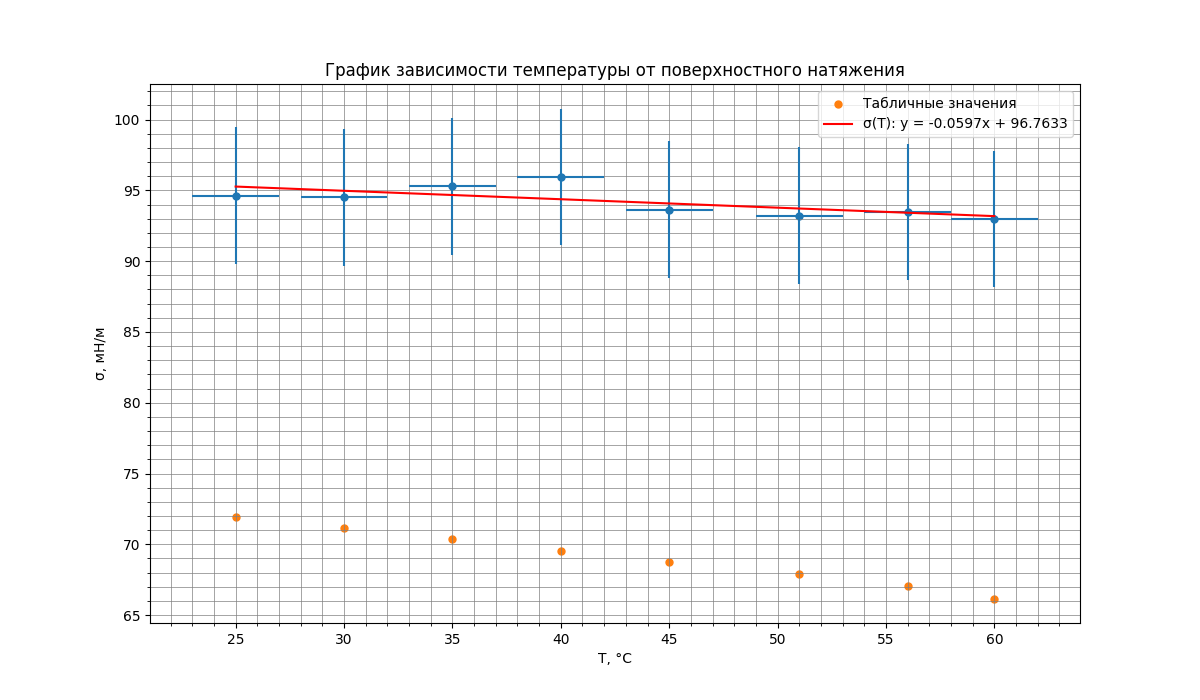
\includegraphics[width=1 \textwidth]{251-1gr.png}
                    \end{center}
                \end{figure}

                Коэффициент наклона графика $k_1 = -0,058$, отсюда мы найдём $\frac{d\sigma}{dT} = k_1 = -0,058$
                \[\sigma_{k_1} = 0,021 \ \text{мН/м} \quad \varepsilon_{\sigma_{k_1}} = 35,87 \%\]
                Такая большая относительная погрешность связана, опять же, с теми условиями, которые перечисленны в пункте 4.3.

                \subsubsection{График зависимости теплоты образования единицы поверхности жидкости и поверхностной энергии U единицы площади F от температуры}

                Коэффициент наклона графика $k_2 = 0,058$
                \[\sigma_{k_1} = 0,021 \ \text{мН/м} \quad \varepsilon_{\sigma_{k_1}} = 35,87 \%\]

                \begin{figure}[!ht]
                    \begin{center}
                        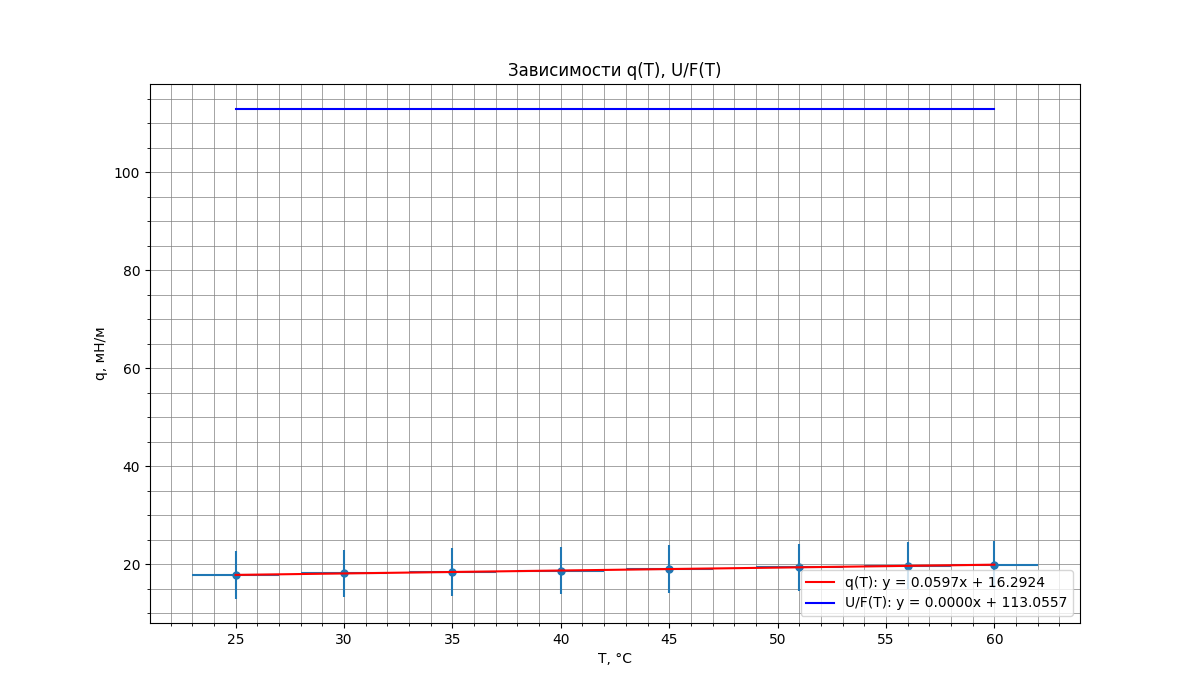
\includegraphics[width=1 \textwidth]{251-2gr.png}
                    \end{center}
                \end{figure}

                На втором графике получили также зависимость поверхностной энергии U единицы площади F от температуры, её коэффициент наклона $k_3 = 0$.
                \section{Выводы}
                \begin{table}[H]
                \centering
                \caption{Сравнение}
                \begin{tabular}{|c|c|c|c|}
                    \hline
                              & $d$, мм & $\Delta h$, мм  \\
                    \hline
                    экспериментальное & 0,938 & 13,5   \\
                    \hline
                    измеренное прибором & 1,05 & 13,5  \\
                    \hline
                \end{tabular}
                \end{table}

            В ходе лабораторной работы мы измерили температурную зависимость коэффициента поверхностного
            натяжения дистиллированной воды, определили полную поверхностную энергию и теплоту, которую необходимую для изотермического образования единицы поверхностного натяжения. 
                Определили эксперименально диаметр иглы, а также измерили его под микроскопом, результаты приведены в таблице 2 выше. 
            Также измерили и посчитали $\Delta h$ двумя способами. Оба измерения полностью совпали. Неточными оказались измерения коэффициента поверхностного натяжения воды, это связано с возможной разностью температур иглы и воды, а также с плохим качеством дистиллята. Для установления равновесия в системе необходимо, чтобы прошло большое количество времени, что также могло повлиять на неточность результата.
    
\end{document}